\documentclass[12pt,times,a4paper]{report}
\setlength{\textwidth}{6.25in}
\setlength{\textheight}{9in}
\renewcommand{\baselinestretch}{1.5}
\oddsidemargin 20pt
\evensidemargin 20pt
\topmargin 0.0pt
\usepackage{hyperref}
\usepackage{fancyhdr}
\usepackage{fancybox}
\usepackage{times}
\usepackage{cite}
\usepackage{graphicx}
\usepackage[left=1.25in,right=1in,top=1in,bottom=1in]{geometry}
\usepackage{hyperref}
\usepackage{amsfonts}
\usepackage{amssymb}
\usepackage{amsmath}
\usepackage{float}
\usepackage{pdfpages}
\usepackage{algorithmic}
\usepackage{algorithm}
\usepackage{comment}
\usepackage{multirow}
\usepackage{titlesec}
\usepackage{lipsum}
\usepackage{graphics}
\usepackage{graphicx}
\usepackage{fancyhdr}
\usepackage{bm,nicefrac}
\titleformat{\chapter}[display]{\Large\bfseries}%
    {\chaptername~\thechapter}{1ex}{}[\titlerule]

% Redefine the plain page style
\pagenumbering{gobble}
 \fancypagestyle{plain}
 
%certificate 
\begin{document}
\begin{titlepage}
\newpage

\pagestyle{empty}
\pagenumbering{Roman}

\thispagestyle{empty}
\thisfancypage{%
  \setlength{\fboxrule}{2pt}\doublebox}{}

\begin{center}
\vspace*{0.2in}
{\fontsize{18}{16} \bf {A}}\\
{\fontsize{18}{16} \bf {Project Based Seminar Report}}\\
{\fontsize{18}{16} \it {On }}\\
\vspace*{0.2in}
{\fontsize{18}{14} \bf {\lq\lq  Prediction of values using Machine Learning Algorithms \rq\rq}}\\
\vspace*{0.2in}
{\fontsize{12}{16} \bf  Submitted to the}\\
{\fontsize{12}{16} \bf Savitribai Phule Pune University
}
\begin{normalsize}
\begin{center}
In partial fulfillment for the award of the Degree of
\end{center}
\end{normalsize}

{\fontsize{14}{12} \bf  Bachelor of Engineering }\\
{\fontsize{14}{12} \bf  In}
\\{\fontsize{14}{12} \bf  Information Technology }\\
{\fontsize{12}{16} \bf   By}\\
\vspace*{0.1in}
{\fontsize{14}{12} \bf Shubham Derhgawen }\\
{\fontsize{12}{8} \bf [Exam seat No T150608505] }\\

\vspace*{0.2in}
{\fontsize{12}{16} \bf Under the Guidance of }\\
\vspace*{0.1in}
{\fontsize{14}{12} \bf Prof. Pooja Kadam}\\
\begin{figure}[h]
\centerline{
\includegraphics[scale=0.8]{logo1.jpg}}
\end{figure}

{ \fontsize{14}{12}  {Department Of Information Technology}}\\
{ \fontsize{14}{12} \bf {Dhole Patil  College Of Engineering}}\\
{ \fontsize{14}{12}  {DHOLE PATIL COLLEGE ENGINEERING, PUNE-412207 (India)}}\\

Academic year 2018-19

\end{center}
\end{titlepage}
%-------------------Cover page ends
%-------------------Certificate Starts


\begin{titlepage}
\begin{center} 
\addcontentsline{toc}{chapter}{Certificate}
\begin{figure}[h]

\centerline{
\includegraphics[scale=0.8]{logo1}}

\end{figure}


\vspace*{0.1in}
{\fontsize{16}{12}\textbf{{CERTIFICATE}} }\\
\begin{enumerate}
\vspace{0.3in}
This is to certify that the project based seminar report entitled \lq\lq \textbf{ “Prediction of values using Machine Learning Algorithms”}
 \rq\rq
being submitted by \textbf{ Shubham Derhgawen (T150608505)}  is a record of bonafide work carried out by him
/her under the supervision and guidance\textbf{ Prof. Pooja Kadam } in partial fulfillment of the
requirement for \textbf{ TE (Information Technology Engineering) – 2015} course of Savitribai Phule
Pune University, Pune in the academic year 2018-2019

\vspace*{0.3in}
Date  : .........................  \\ 
Place : .........................  \\ 
 
\vspace{0.8in}
\begin{table} [h]
\addtolength{\tabcolsep}{65pt}
\begin{tabular}{c                c  }
Seminar Guide  & H.O.D \\
 Prof. Pooja Kadam  & Prof. Ameet Zore 
\end{tabular}
\end{table}
\vspace{0.8in}

This project-based seminar report has been examined by us as per the Savirtibai Phule Pune
University, Pune, requirements at Dhole Patil College of Engineering on . . . . . . . . . . . ..
\begin{table} [h]
\addtolength{\tabcolsep}{65pt}
\begin{tabular}{c                c  }
Name \& Sign  & Name \& Sign \\
 Internal Examiner   & External Examiner 
\end{tabular}
\end{table}
\end{enumerate}
\end{center}

\end{titlepage}
%-------------------Certificate Ends
%-------------------Acknowledgement Starts
%\begin{titlepage}
\newpage
\begin{center}
\pagenumbering{roman}
\thispagestyle{empty}
\renewcommand{\baselinestretch}{1.5}
\addcontentsline{toc}{chapter}{Acknowledgement}
{\fontsize{12}{10} \bf ACKNOWLEDGEMENT}\\
%\section{ACKNOWLEDGMENT}
\begin{enumerate}
\vspace{0.4in}
The completion of report on \textbf{“Prediction of values using Machine Learning Algorithms”} has given me immense pleasure and knowledge. I am sincerely thankful to Principal \textbf{Dr. N. Walimbe , Prof. Amit Zore} our head of the IT Department, project based seminar guide \textbf{Prof. Pooja Kadam } and project based seminar in charge \textbf{Prof. Rahul Ghode} who have cooperated with me at different stages during the preparation of this report.

My sincere thanks to the staff of Information Technologies Department without whose help it
would not have been possible for me to complete this report. This work is virtually the result of
inspiration given by them.

I would also like to thank all the library and non teaching staff for their help and last but not
least, I would like to thank all my friend for their constant help and support.

\end{enumerate}
\end{center}
\vspace*{0.8in}
{\bf Shubham Derhgawen}\\

%\end{titlepage}
%-------------------Acknowledgement Ends

%-------------------List of publication Starts
%\begin{titlepage}
\newpage

%-------------------List of publication Ends

%-------------------List of Figures starts
\newpage






%-------------------List of Figures ends

%-------------------List of tables starts

%-------------------List of table ends

%-------------------List of Abrevations starts


%-------------------List of Abrevations ends

%-------------------Abstract Starts
%\begin{titlepage}

\newpage





%-------------------List of Figures ends

%-------------------List of tables starts

%-------------------List of table ends

%-------------------List of Abrevations starts


%-------------------List of Abrevations ends

%-------------------Abstract Starts
%\begin{titlepage}


\newpage
\renewcommand{\baselinestretch}{1.5}

\addcontentsline{toc}{chapter}{Abstract}
\begin{center}
{\fontsize{14}{12} \bf ABSTRACT}\\

\begin{enumerate}
\begin{normalsize}
\vspace{0.4in}
              The smart management water for maximum use and minimum wastage is essential for reducing the water crisis that the world faces today, all the while contributing to environmental sustainability. The intense use of technologies offers a means for providing the exact amount of water needed for each purpose and use and not a drop more. 
The Internet of Things (IoT) is the natural choice for smart water management applications, even though the integration of different technologies required for making it work seamlessly in practice is still not fully accomplished. The SMART2L project develops an IoT-based smart water management platform to curb the problem of water crisis and manage water resources efficiently with a hands-on approach. 
This paper presents a study about IoT that stands to change dramatically the way it impacts on the water crisis in the world. this paper also presents the perspective on the challenges of SMART2L in delivering its service to provide the assistance in solving water crisis especially in managing water resources.
\\

\end{normalsize}
\end{enumerate}
\end{center}
%\end{titlepage}
%-------------------Abstract ends

%--------------------------------- Table of Contents
	
\newpage
\thispagestyle{empty}
\renewcommand{\baselinestretch}{1.5}
\begin{normalsize}

\renewcommand{\headrulewidth}{0pt}
\renewcommand{\footrulewidth}{0pt}
\tableofcontents 
\end{normalsize}


\newpage
\addcontentsline{toc}{chapter}{List of Figures}
\thispagestyle{empty}
\renewcommand{\baselinestretch}{1.5}

 {\setlength{\baselineskip}{1.5\baselineskip}
\fontsize{16}{14}
\listoffigures
\addcontentsline{toc}{chapter}{LIST Of FIGURES}


\renewcommand{\headrulewidth}{0.4pt}
\renewcommand{\footrulewidth}{0.4pt}
\pagenumbering{arabic}
\fancyhf{} %reset header and footer
 \pagestyle{fancy}
 \fancyhead[R]{Prediction of values using Machine Learning Algorithms}
\fancyfoot[R]{ \thepage}
\fancyfoot[L]{ Department of Information Technology, DPCOE, Pune }


\newcommand{\cchapter}[1]{\chapter[#1]{\centering #1}}
{\setlength{\baselineskip}{\baselineskip}
\begin{center}
  \chapter{\fontsize{12}{14}\textbf{Introduction to Prediction of values using Machine Learning Algorithms \hfill}}  
\end{center}
\section{Introduction }
\begin{normalsize}
\par
With the ever increasing amounts of data becoming
available there is good reason to believe that smart data analysis will become
even more pervasive as a necessary ingredient for technological progress. 
When the amount of data available is enormous, it helps if some of the analysis can be automated. Machine learning is a way of identifying patterns in data and using them to automatically make predictions or decisions. 
The age of Big Data gives us a lot to learn from. This abundance of data can be used in various fields to make decisions based on predictions. But different characteristics of data present us with challenges of varied difficulties . Each case different from others . To overcome 
this challenge we study various algorithms and their abilities to solve each problem of prediction. Our project focuses on studying different algorithms for prediction and comparison of each one of them. 
\par
The time of using machine learning is right only when there is abundance of data to learn from. As the time is right , it gives us the opportunity to work on it and produce mathematical models for prediction with ease. Often the accuracy of models is said to be highly dependent on amount of data but proper use of it is equally helpful in improving it. In today's day , need of prediction  has become quite important and systems which could tell the confidence of these predictions help even more to solve business decision problems and other such problems related to other industries such as health care and finance.
\newpage
\section{Motivation}

Predictions based on machine learning models today help in making making big business decisions or even predicting the effectiveness of a drug on a patient .This helps society in numerous ways , improving the stock markets by predicting their values or saving lives by predicting which drug affects the patient the best.
\section{Aim and Objective(s) of the work}
The aims of this project are:
\begin{itemize}
    \item Understand existing methods and algorithms for prediction. And find their advantages/disadvantages.
    \item Test the different  algorithms on different parameters. 
    \item Improving the performance of existing algorithms.
    \item Explore new use cases for the algorithms and use the knowledge to build a solution for everyday world.
\end{itemize}
The objectives of this project are:
\begin{itemize}
    \item[1.]To understand existing algorithms we study and build them from scratch in a generic programming language.
    \item[2.]To test the algorithms we find different performance parameters.
    \item[3.]To improve on their existing performance by tweaking them to suit the data.
    \item[4.]To find new use cases we study problems if different disciplines.
\end{itemize}
\newpage
\section{Introduction to IOT to minimize water crisis }
Water utilities in world are still marching at a greatly deliberate speed when it comes to deal with smart water management. Not anything like gas and electricity, most are in synchronized with the adopted cutting-edge technology. As an IoT solution, SMART2L can play its part in the current developing industry like the new housing development, in supporting the government’s policy on focusing the latest knowledge and technology on water management to ensure sustainable water development resources .  
Mutual real-time data is a smarter pronouncement . Data collected can be promptly turned into valued data for any reasonable decision making in the entire areas of the company, improving the whole part of the utility's data sharing technique that is normal for daily tasks. Eventually, operators, planners, and managers can obtain continuous, pertinent and precise updates anytime from everywhere despite the need to wait for offline reports or data. 
\subsection{Aim and Objectives of Seminar}
\begin{itemize}
    \item \textbf{Preservation and Protection of Our Natural Resources:} Conserving water can help preserve our natural resources. Conserving water means more water is available to serve additional water needs, as well as for wildlife and recreation. 
    \item \textbf{Saving Money for Our Citizens and Our Community :}Conserving water can reduce the amount of money spent each month for household water use
 \item\textbf{Insuring the Reliability of Our Water Supply :} Water conservation can positively affect the reliability of our water supply during periods of high demands (such as the summer months) and during droughts. 
\item \textbf{Use of IOT to maximize efficient utilization of water.}
\end{itemize}
\newpage
\chapter{\fontsize{18}{16}\textbf{LITERATURE SURVEY}}

\begin{itemize}
\item[[1]]\textbf{Paper Title:} "IOT based Water Management".
\par
\textbf{Publish Year}:March,2017
\par
\textbf{Rescorces/Facilities Used:}
\begin{itemize}
    \item 	Water resources,
	\item Cloud computing,
\item Internet of Things,
\item Mobile applications,
\item Magnetic sensors,
\item Rotors
\end{itemize}
\item[[2]]\textbf{Paper Title:} "Smart water management using IOT".
\par
\textbf{Publish Year}:2016
\par
\textbf{Rescorces/Facilities Used:}
\begin{itemize}
    \item Wireless fidelity
\item Cloud computing,
\item Internet of Things,
\item Mobile applications,
\item Magnetic sensors
\item Pins
\end{itemize}
\item[[3]]\textbf{Paper Title:} "Self powered IOT-enabled water monitoring system".
\par
\textbf{Publish Year}:2018
\par
\textbf{Rescorces/Facilities Used:}
\begin{itemize}
    \item 	Wireless communication
\item	Cloud computing,
\item	Internet of Things,
\item	Mobile applications,
\item	Wireless sensor network,
\item	Temperature measurement
\end{itemize}
\end{itemize}
\par
\textbf{Advance Research:}
\par
All the above research papers have their pros and cons , on the basis of these this project aims to eliminate the disadvantages and glorify the advantages. The difference being not just in managing the water resources or monitoring them but also in taking instant action, reducing wastage an curbing the water crisis.The modernization of monitoring using apps and instant action options furthermore have a humungous effect on the reduction of water wastage. The use of IOT helps in minimizing the error , efforts and improves accuracy of monitoring and response. 


\chapter{\fontsize{16}{14}\textbf{Perceptron\hfill}}

\section{Introduction}

\par
The most fundamental unit of a deep neural network is called an artificial neuron, which takes an input, processes it, passes it through an activation function like the Sigmoid and returns the activated output.Frank Rosenblatt, an American psychologist, proposed the classical perceptron model in 1958. Further refined and carefully analyzed by Minsky and Papert in 1969 in their model is referred to as the perceptron model.

\begin{figure}[H]
\begin{center}
\fbox{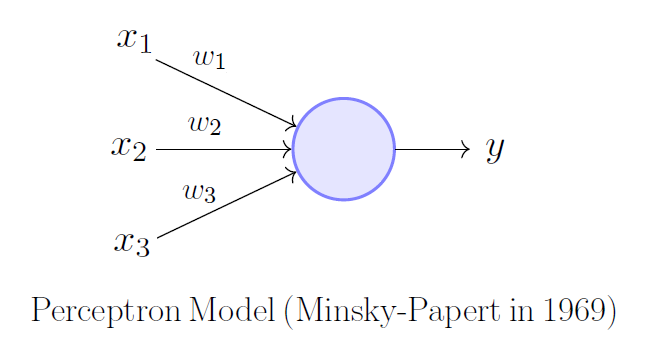
\includegraphics[width=8cm]{percep.png}}
\end{center}
\end{figure}

\section{Definition}
The perceptron is an algorithm for supervised learning of binary classifiers. the perceptron is an algorithm for learning a binary classifier called a threshold function: a function that maps its input $\mathbf {x}$  (a real-valued vector) to an output value $ f(\mathbf {x} )$ (a single binary value):
$f(\mathbf{x})=\left\{\begin{array}{ll}{1} & {\text { if } \mathbf{w} \cdot \mathbf{x}+b>0} \\ {0} & {\text { otherwise }}\end{array}\right.$\\
where $ \mathbf {w}$  is a vector of real-valued weights,$ {\displaystyle \mathbf {w} \cdot \mathbf {x} }$ is the dot product$ {\displaystyle \sum _{i=1}^{m}w_{i}x_{i}} $where m is the number of inputs to the perceptron, and b is the bias. The bias shifts the decision boundary away from the origin and does not depend on any input value.

\newpage
The information gathered from the real-time monitoring will be benefited department of water resources and also the public. The main idea of a real-time IOT-based water resources information system is to convey inclusive and precise figures
\begin{figure}
\begin{center}
\fbox{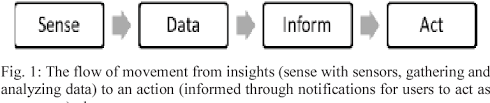
\includegraphics[width=10cm]{fig_01.png}}
\caption{\text{Real-time IOT-based water resources Information System }}
\end{center}
\end{figure}
\pagebreak
\section{How it Works?}
\par
SMART2L system integrates the usage of Arduino Yun. A reserve tank, batteries (power supply), water tank and water pump are used to set up the water pump system. The reserve tank is connected to the main tank via a water pump. The water pump is used to pump water from reserve to the main tank and is controlled by the main tank’s water threshold, which turns on/off the water pump. This is the most common method of threshold level control for the main tank which simply to start the water pump at its low level and permits it to run until the water is filled up.

\begin{figure}
\begin{center}
\fbox{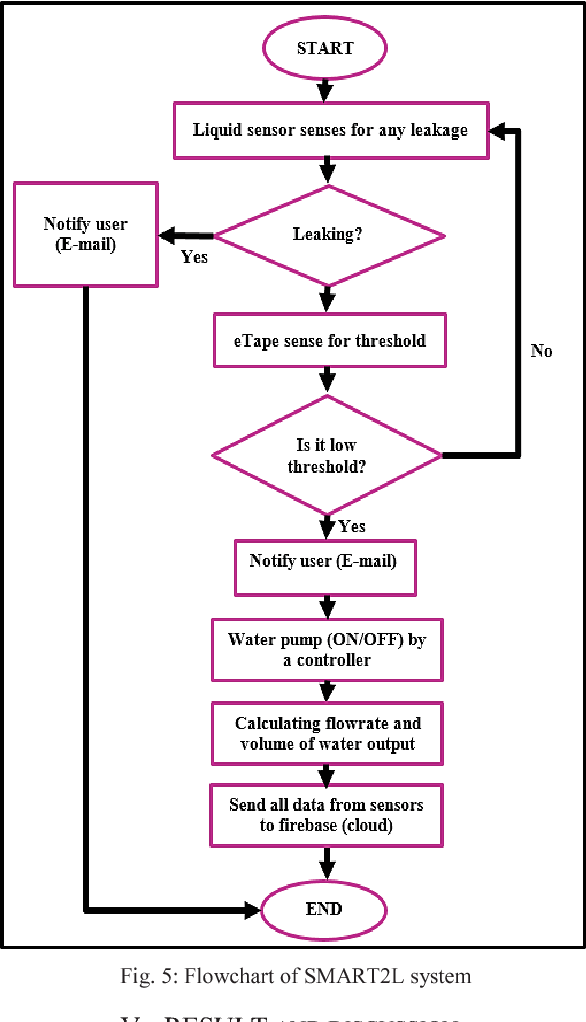
\includegraphics[width=8cm]{fig.png}}
\caption{\text{Flow of Real-time IOT-based water resources Information System }}
\end{center}
\end{figure}

\begin{figure}
\begin{center}
\fbox{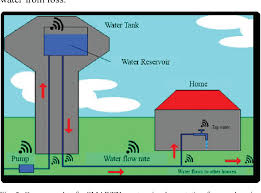
\includegraphics[width=10cm]{fig_03.jpg}}
\caption{\text{Model of Real-time IOT-based water resources Information System }}
\end{center}
\end{figure}
\pagebreak
\begin{itemize}
    \item[A.]\textbf{Presence of Leaks}
    \par
    The liquid sensor will first sense any leakage present either at the valve or the distribution of PVC pipes. If there is a presence of leakage, the Arduino Yun will send an e-mail to notify the users. The decrease in the water below the threshold level will cause Arduino Yun to send an e-mail too. This will cause the pump to automatically pump water and liquid will start to flow from the reservoir to the main tank till it is full. Beforehand, users need to install the SMART2L apps on their smartphone to ensure the users able to monitor SMART2L system through mobile apps as Arduino Yun sends the system data to Firebase.
\begin{figure}
\begin{center}
\fbox{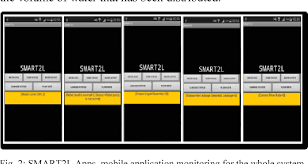
\includegraphics[width=8cm]{fig_02.png}}
\caption{\text{Mobile Based Application for  IOT-based water resources Information System }}
\end{center}
\end{figure}
\newpage
    \item[B.]\textbf{The absence of Leaks; Low Threshold}
On the other hand, in the absence of leakage                    the SMART2L  system continuously still sense the liquid threshold through eTape sensor. Any changes, Arduino Yun will send notification through e-mail. Simultaneously, the shape sensor monitors the threshold level as a step taken to prevent the liquid from overflowing. Real-time data will continuously be updated to Firebase.
The information of the SMART2L system that is gathered in Firebase to view overall data. The data will be constantly updated in the real-time following any changes happen within the system. Firebase is used together to store the analytics info gathered from all the available sensors in the SMART2L system. The information in Firebase is stored in JSON format. Every updated, added or deleted information can be observed in real-time and colors flashing in the cloud database based on Fig.3.5 signifying such actions are being done. 
\begin{figure}
\begin{center}
\fbox{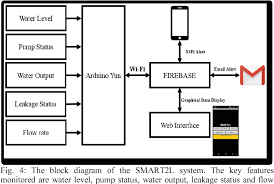
\includegraphics[width=10cm]{fig_04.png}}
\caption{\text{Block Diagram of Smart2L }}
\end{center}
\end{figure}
\end{itemize}
\par
Apart from that, the users will also receive an email notification on alerting the users about the water threshold as well as if any leakage present.
\begin{figure}
\begin{center}
\fbox{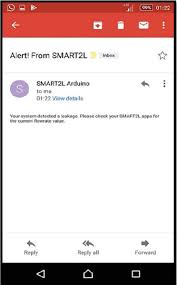
\includegraphics[width=8cm]{fig_05.jpg}}
\caption{\text{Email Alert }}
\end{center}
\end{figure}
\pagebreak

\chapter{\fontsize{16}{14}\textbf{CONCLUSION}}

\par
Investing in the current cutting-edge technology like the Internet of Things (IoT) really gives great impact in curbing the issues related to the water crisis and water management. The existing systems employ additional period to gather data and focus less on the insights of the data. Most of the existing systems require the manual collection of data. 
\par
The SMART2L monitoring system, an IoT-based system able to deliver a better solution in monitoring the water resources which equipped with proper sensors. A faulty pipe can leak anywhere within seconds. Without proper flow sensor monitoring on sites, a basic break like this could be resulted in losing substantial amounts of water and can take weeks to be made conscious of the matter
\par
  This real-time visibility and remote access have been so beneficial to the district, that SMART2L system has can now become mandatory especially for all new construction projects.. 
\par
Beside that this project can be implemented in a real situation and can hold a market value especially in a residential unit or in industries. This is because it is about time for the residential and also the industry to make a change to appreciate the benefits of IoT since they still reliably engaged to the float technology which marginally inefficient and lacking precisions.

\newpage
\clearpage
%\chapter{\fontsize{16}{14}\textbf{REFERENCES}}
\begin{flushright}
\begin{center}
\fontsize{16}{14}\textbf{REFERENCES}
\end{center}
\end{flushright}
%\section*{REFERENCES}
\addcontentsline{toc}{section}{REFERENCES}
%\textbf{Base Paper:}
\begin{normalsize}

\end{normalsize}
\begin{itemize}
\item[[1]] S. M. Shahabudin. Water Malaysia 2015. (2), 3-22. 
\end{itemize}
%\textbf{Reference Papers:}
\begin{itemize}
\item[[2]]H. Harun, Water Crisis is real, Zahid wants industry players to use tech, innovation to better manage water resources. Kuala Lumpur: The New Straits Times 
\item[[3]]Bernama. Selangor to face critical water shortage from 2017-2019, MB says. Kuala Lumpur: The Malay Mail Online. 
\item[[4]]  F. F. Zulzaha. Suggestions for residents and Syabas on ways to counter water shortage. Kuala Lumpur: starproperty.my. 

\item[[5]]J. M. Choong. Industries Fear Nation's Worst Water Crisis. Petaling Jaya: The Malay Mail Online.

\item[[6]] Lai C.H., Phang W.L., and Chan N.W. (2013). A Study of Non-Revenue Water Management in Penang as an Example of Good Water Governance. 

\item[[7]]M. D. Chow. M'sia Targets 'Non-Revenue Water' Reduction of 25 Percent by 2020: Water Ministry. Kuala Lumpur: The New Straits Times Online. 
\end{itemize}

\end{normalsize}
\end{document}